\documentclass{sciposter}
\usepackage{lipsum}
\usepackage{listings}
\usepackage{epsfig}
\usepackage{amsmath}
\usepackage{amssymb}
\usepackage{multicol}
\usepackage{graphicx,url}
\usepackage[portuges, brazil]{babel}   
\usepackage[utf8]{inputenc}

\newtheorem{Def}{Definition}


\title{Projeto Interativo III\\ Angry Robots}


\author{Caroline Bomfim do Espirito Santo, Mahaira Soares de Souza, Rafael da Silva Santos, Thiago de Sousa Messias}


\institute 
{Bacharelado em Ciência da Computação\\
Centro Universitário SENAC - Campus Santo Amaro
(SENAC-SP)\\
Av. Engenheiro Eusébio Stevaux, 823 -- Santo Amaro, São Paulo -- CEP 04696-000 -- SP -- Brasil}


\email{caroline.bomfim@hotmail.com.br, mahaira\_souza@hotmail.com, rafa\_silva.santos@hotmail.com, messiasthi@gmail.com}

\leftlogo[1]{Senac-logo}
\rightlogo[2]{bcc-logo}

\begin{document}

\conference{{\bf PI III}- Senac, 05 de Maio de 2014, São Paulo, Brasil}

\maketitle

\begin{multicols}{3}
\section {Resumo}

Angry Robots é um jogo desenvolvido em linguagem C, ultilizando a biblioteca gráfica allegro 5, fundamentado em visão computacional "OpenCV". Um de seus principais objetivos é induzir a atividade física, fazendo com que o usuário se movimente para conseguir derrotar um robô, a parte de visão computacional foi construida com algotitmos em função do cálculo da centróide e o sistema de cores HSV (formado pelas componentes Hue (tonalidade), Saturation (saturação) e Value (valor).

\begin{figure}[!htb]
\centering
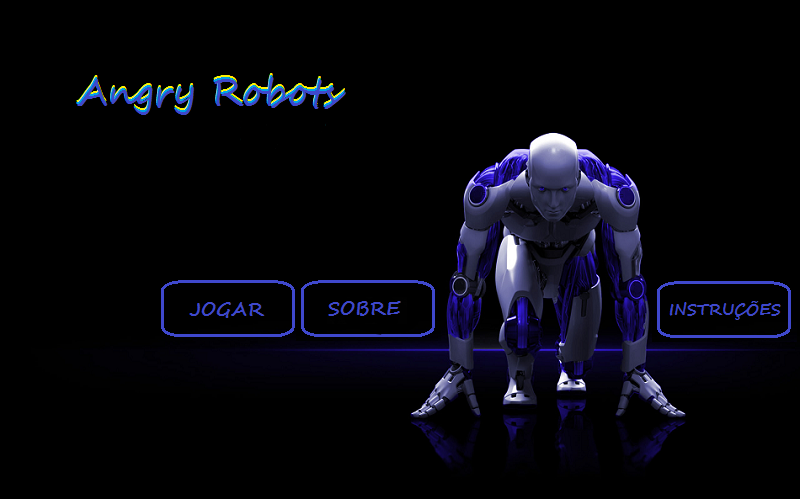
\includegraphics[scale=0.8]{menu.png}
\caption{Versão beta do jogo, com design teste.}
\end{figure}


\section{Introducão}
Nos últimos anos a industria de jogos cresceu de forma constante, e com ela a importância dos mesmos para o desenvolvimento de muitas habilidades. 
Angry Robots, o mesmo induz que o jogador se movimente de forma rápida e lógica para que consiga chegar ao objetivo final, ganhar a partida e derrotar o robô.
Quando tratado à imagem é utilizado algoritimos e fórmulas matemáticas, inclusive e principalmente a física para que seja calculado a fraquencia e tonalidade de cores de cada pixel's, iluminação e luminosidade do local, tanto para sabermos em qual escala de cor ele se encontra, quanto para melhorar a qualidade visual.

\begin{figure}[!htb]
\centering
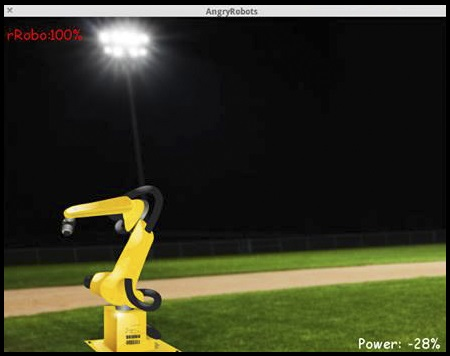
\includegraphics[scale=1.4]{betateste.jpg}
\caption{Versão beta do jogo, com design teste.}
\end{figure}

\vspace{0.7cm}

\newcommand{\imsize}{0.45\columnwidth}

\section{Revisão de Literatura}
Angry Robots é um jogo limitado, pois dentro dos requisitos fora permitidos somente as bibliotecas, allegro 5 gráfica e a multiplataforma OpenCV utilizada para desenvolvimento de aplicativos na área de visão computacional.
Existem diversos jogos em que o Angry Robots foi baseado, como no Cube Slam, um jogo que os usuários se enfrentam em uma partida visual de air hockey, onde o jogador luta contra um urso, no caso do Angry Robots o adversário é o robô rápido e inteligente. Também existiam projetos no blog "Laboratório Garagem", entretanto todos fugiam do ambiente proposto, a maioria deles utilizavam Arduíno, OpenCV e Python, mesmo com os obstáculos foi de grande utilidade pois algumas ideias surgiram através de post's referentes à robôs. Gran Slam Tennis 2, foi utilizado em questão dos movimentos do jogo, e o enredo em si, do MechWarrior. Os algorítimos desenvolvidos são autorais sem base em outros jogos, visto que mesmo com fundamento em tantos jogos, Angry Robots é um diferencial de jogos.

\section{Desenvolvimentos}

\textbf{Centróide} 
é nome dado ao ponto interior que define seu centro geométrico. Caso a forma geométrica represente uma secção homogénea de um corpo, então o centróide coincide com o centro de massa. Nos casos em que não só o corpo é homogéneo e está submetido a um campo gravítico constante, então esse ponto coincide com o centro de gravidade. A centróide e implementada no código para captar o meio da tela, facilitando a detecção do resto da tela para variação é identificação da cor de preferência.

\begin{figure}[!htb]
\centering
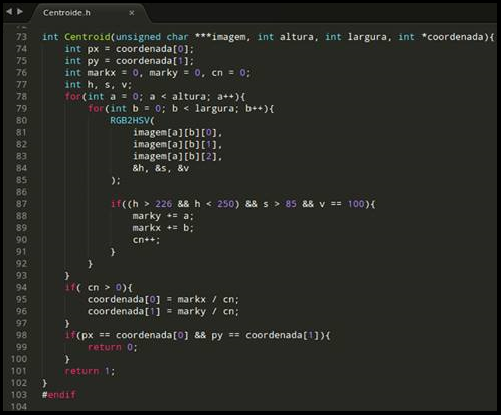
\includegraphics[scale=1.7]{centroid.png}
\caption{Exemplo: Código Centróide.}
\end{figure}


\textbf{Conversão para HSV}
calcula a intensidade da tonalidade, saturação e brilho da imagem, isto possibilitou um aprimoramento no rastremento do jogo, pois a iluminação, e os objetos ao redor poderão ser ignorados, não atrapalhando a jogabilidade. A tonalidade permite distinguir as cores puras de 0 á 360 graus, a saturação verifica a intensidade da pureza da tonalidade, o brilho verifica a iluminação da imagem.

\begin{figure}[!htb]
\centering
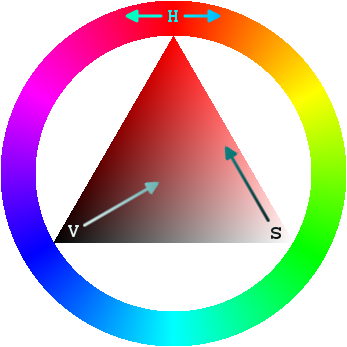
\includegraphics[scale=0.7]{Triangulo_HSV.png}
\caption{Exemplo: triangulo de explicação HSV }
\end{figure}

\textbf{Ponto de maior reflexão de pixels}

\textbf{Nivel de saturação}
 
\textbf{Histograma}

Em estatística, um histograma , também conhecido como distribuição de frequências ou diagrama das frequências, é uma representação gráfica na qual um conjunto de dados é agrupado em classes uniformes, representado por um retângulo cuja base horizontal são as classes e seu intervalo e a altura vertical representa a frequência com que os valores desta classe estão presente no conjunto de dados.

\section{Resultados }

Neste jogo o robô ira tentar fugir para que o jogador não consiga acerta-lo com pequenas bolas, 
isto será feito através de um laser azul, o objetivo do jogo é derrotar o robô jogando as bolas em sua direção, quanto mais rápido os movimentos do usuário, mais chances de vencer o jogo.

\vspace{0.7cm}

\begin{figure}[!htb]
\centering
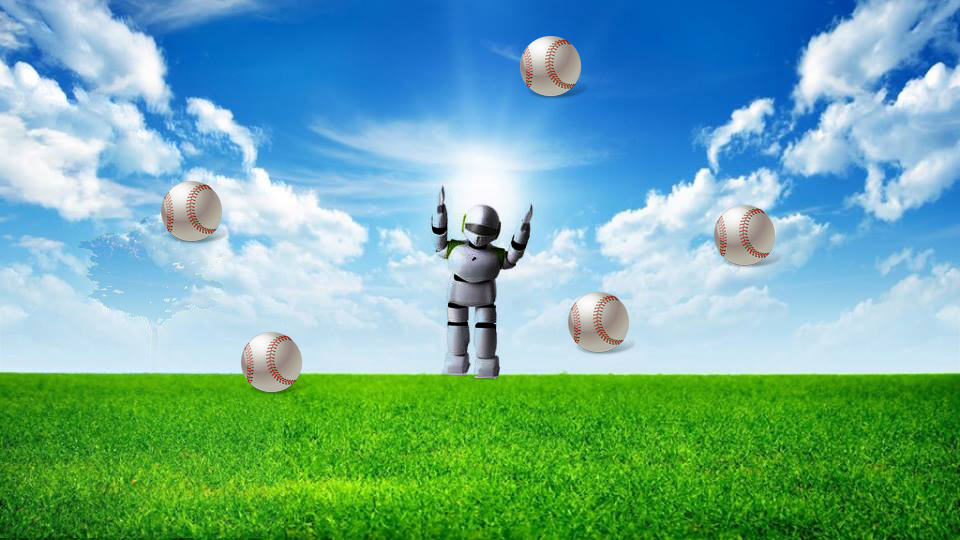
\includegraphics[scale=0.7]{fundo.jpg}
\caption{Imagem do jogo funcionando}
\end{figure}

\section{Considerações Finais}

O rastreamento é o ponto mais difícil, pois alguns fatores atrapalharam o desenvolvimento do mesmo, um deles foi a iluminação, pois devido a ela, a imagem pode ser ofuscada ou obscurecida demais, porém o HSV permitiu que a iluminação fosse ignorada, pois este algoritmo converte toda a imagem para cinza, e trata a variação da luminosidade, deste modo o usuário poderá jogar com uma camiseta azul por exemplo, sem afetar o rastreamento.


\bibliographystyle{plain}
\begin{thebibliography}{5}

\bibitem{site r7}  Portal R7 de notícias 
\\
\newblock http://noticias.r7.com/tecnologia-e-ciencia/noticias/jovens-apelam-para-games-corporais-para-melhorar-condicionamento-fisico-20110527.html


\bibitem{livro}
H. M. Deitel e P. J. Deitel.
\newblock Como programar em C, 2º edição.

\bibitem{site allegro} http://www.rafaeltoledo.net/tutoriais-allegro-5/
\\
\newblock Allegro 5.

\bibitem{site opencv} http://opencv.org/
\\
\newblock OpenCv

\bibitem{site rgb} http://www.rapidtables.com/web/color/RGB\_Color.htm \\
\newblock RGB


\end{thebibliography}

\end{multicols}

\end{document}

